% This is "sig-alternate.tex" V2.0 May 2012
% This file should be compiled with V2.5 of "sig-alternate.cls" May 2012
%
% This example file demonstrates the use of the 'sig-alternate.cls'
% V2.5 LaTeX2e document class file. It is for those submitting
% articles to ACM Conference Proceedings WHO DO NOT WISH TO
% STRICTLY ADHERE TO THE SIGS (PUBS-BOARD-ENDORSED) STYLE.
% The 'sig-alternate.cls' file will produce a similar-looking,
% albeit, 'tighter' paper resulting in, invariably, fewer pages.
%
% ----------------------------------------------------------------------------------------------------------------
% This .tex file (and associated .cls V2.5) produces:
%       1) The Permission Statement
%       2) The Conference (location) Info information
%       3) The Copyright Line with ACM data
%       4) NO page numbers
%
% as against the acm_proc_article-sp.cls file which
% DOES NOT produce 1) thru' 3) above.
%
% Using 'sig-alternate.cls' you have control, however, from within
% the source .tex file, over both the CopyrightYear
% (defaulted to 200X) and the ACM Copyright Data
% (defaulted to X-XXXXX-XX-X/XX/XX).
% e.g.
% \CopyrightYear{2007} will cause 2007 to appear in the copyright line.
% \crdata{0-12345-67-8/90/12} will cause 0-12345-67-8/90/12 to appear in the copyright line.
%
% ---------------------------------------------------------------------------------------------------------------
% This .tex source is an example which *does* use
% the .bib file (from which the .bbl file % is produced).
% REMEMBER HOWEVER: After having produced the .bbl file,
% and prior to final submission, you *NEED* to 'insert'
% your .bbl file into your source .tex file so as to provide
% ONE 'self-contained' source file.
%
% ================= IF YOU HAVE QUESTIONS =======================
% Questions regarding the SIGS styles, SIGS policies and
% procedures, Conferences etc. should be sent to
% Adrienne Griscti (griscti@acm.org)
%
% Technical questions _only_ to
% Gerald Murray (murray@hq.acm.org)
% ===============================================================
%
% For tracking purposes - this is V2.0 - May 2012

\documentclass{sig-alternate}

\begin{document}
%
% --- Author Metadata here ---
\conferenceinfo{WOODSTOCK}{'97 El Paso, Texas USA}
%\CopyrightYear{2007} % Allows default copyright year (20XX) to be over-ridden - IF NEED BE.
%\crdata{0-12345-67-8/90/01}  % Allows default copyright data (0-89791-88-6/97/05) to be over-ridden - IF NEED BE.
% --- End of Author Metadata ---

\title{Identifying MFSs with considering masking effect\titlenote{(Does NOT produce the permission block, copyright information nor page numbering). For use with ACM\_PROC\_ARTICLE-SP.CLS. Supported by ACM.}}
\subtitle{[Extended Abstract]
\titlenote{A full version of this paper is available as
\textit{Author's Guide to Preparing ACM SIG Proceedings Using
\LaTeX$2_\epsilon$\ and BibTeX} at
\texttt{www.acm.org/eaddress.htm}}}
%
% You need the command \numberofauthors to handle the 'placement
% and alignment' of the authors beneath the title.
%
% For aesthetic reasons, we recommend 'three authors at a time'
% i.e. three 'name/affiliation blocks' be placed beneath the title.
%
% NOTE: You are NOT restricted in how many 'rows' of
% "name/affiliations" may appear. We just ask that you restrict
% the number of 'columns' to three.
%
% Because of the available 'opening page real-estate'
% we ask you to refrain from putting more than six authors
% (two rows with three columns) beneath the article title.
% More than six makes the first-page appear very cluttered indeed.
%
% Use the \alignauthor commands to handle the names
% and affiliations for an 'aesthetic maximum' of six authors.
% Add names, affiliations, addresses for
% the seventh etc. author(s) as the argument for the
% \additionalauthors command.
% These 'additional authors' will be output/set for you
% without further effort on your part as the last section in
% the body of your article BEFORE References or any Appendices.

\numberofauthors{8} %  in this sample file, there are a *total*
% of EIGHT authors. SIX appear on the 'first-page' (for formatting
% reasons) and the remaining two appear in the \additionalauthors section.
%
\author{
% You can go ahead and credit any number of authors here,
% e.g. one 'row of three' or two rows (consisting of one row of three
% and a second row of one, two or three).
%
% The command \alignauthor (no curly braces needed) should
% precede each author name, affiliation/snail-mail address and
% e-mail address. Additionally, tag each line of
% affiliation/address with \affaddr, and tag the
% e-mail address with \email.
%
% 1st. author
\alignauthor
Xintao Niu\\
       \affaddr{State Key Laboratory for Novel Software Technology}\\
       \affaddr{Nanjing University}\\
       \affaddr{China, 210093}\\
       \email{niuxintao@smail.nju.edu.cn}
% 2nd. author
\alignauthor
Changhai Nie\\
       \affaddr{State Key Laboratory for Novel Software Technology}\\
       \affaddr{Nanjing University}\\
       \affaddr{China, 210093}\\
       \email{changhainie@nju.edu.cn}
% 3rd. author
\alignauthor Alvin Chain\\
       \affaddr{Department of computing}\\
       \affaddr{Hong Kong Polytechnic University}\\
       \affaddr{Hong Kong}\\
       \email{cstschan@comp.polyu.edu.hk}
}
% There's nothing stopping you putting the seventh, eighth, etc.
% author on the opening page (as the 'third row') but we ask,
% for aesthetic reasons that you place these 'additional authors'
% in the \additional authors block, viz.
\additionalauthors{Additional authors: John Smith (The Th{\o}rv{\"a}ld Group,
email: {\texttt{jsmith@affiliation.org}}) and Julius P.~Kumquat
(The Kumquat Consortium, email: {\texttt{jpkumquat@consortium.net}}).}
\date{30 July 1999}
% Just remember to make sure that the TOTAL number of authors
% is the number that will appear on the first page PLUS the
% number that will appear in the \additionalauthors section.
\maketitle
\begin{abstract}
Minimal failure-inducing schema(MFS) is a important concept in combinatorial testing that indicate the failure-inducing interaction of parameters in the software under test(SUT). Identify the MFS can help developers quickly reduce the search space needed to find the buggy source. Many algorithms are proposed to find these MFSs in the failing test cases. In practice, however, we find that these algorithms cannot behave as expected in the condition that SUT has multiple faults with different levels. For if so, a fault with higher level may be triggered and leaving the code which will trigger the fault with lower level not executed. Thus we cannot observe the fault with lower level, as a result, we will omit the MFS that related to the fault with lower level. We call this a masking effect.

In this paper, we propose a framework which can help the algorithms to avoid this masking effect when identify MFSs in the test cases. In this framework, we first static analysis the data flow of the test cases. Second we record fault as well as the code lines related to this fault during executing test cases. Then we will determine the levels of different faults we triggered during testing through finding the relationships of the code lines of each fault. By doing so we can judge whether a masking effect is happened during the process of identifying MFS and avoiding them by generating new test case that exposing the fault with lower level.We have applied our framework into several algorithms which focus on identifying the MFS in test cases and empirically studied the framework on two widely used open source software. Our result of the studies shows that our framework can effectively reduce the influence of masking effect.
\end{abstract}

% A category with the (minimum) three required fields
\category{H.4}{Information Systems Applications}{Miscellaneous}
%A category including the fourth, optional field follows...
\category{D.2.8}{Software Engineering}{Metrics}[complexity measures, performance measures]

\terms{Theory}

\keywords{Minimal failure-inducing schemas, Masking effect} % NOT required for Proceedings

\section{Introduction}
With the increase of requirements for more features and customisable, modern software are designed to be configurable and modular. While it can make software portable and flexible, it also bring many challenges to the testers when testing them. The major one of these challenges is that we must make sure the components or options in the software coexistence with each other. As exhaustive testing each possible combination is not impractical when there are large amount of components or options in the SUT, we should choose some of them to test with considering the cost. There are many strategies for one to select the test configurations among all the possible configurations. Combinatorial testing is one of them that can reach the coverage of all the interactions of components with the number of component(we called interaction strength) not more than t.

Which criteria we should choose or how to generate these test cases is not the point in this paper, however, we will focus on the followed problem: if we find some test configurations failed during executing, which subset of the combination of component is the source of this failure?  In another word, we want to identify the failure-inducing interactions of component rather than just detect them. Many works (as well as our previous work) are proposed to solve this problem. Most of these works focus on how to identify as more MFSs as possible while just generating small size of extra test configurations.

In our recent studies, however, we find these algorithms cannot behave as expected in some subject software. Through a deep analysis, we find that there are multiple faults with different levels in these subject. It means that when we set up a test configuration and execute the SUT to observe the result, the high level fault will trigger first and perturb we examining the code that may trigger the low level fault. As a result we will omit some options or component in this test configuration that may be the cause of the low level fault. We call this a masking effect which make the MFS identifying algorithms not able to work properly.

In this paper, we propose a approach that can assist these algorithms to avoid these masking effect. Our framework consists of three parts: first, it will use the statistic analysis technique--dominate tree to analysis the test script and then collect the information
traditional identifying algorithms. of code lines in this script. Second, we will support a interface called "Record" for the MFS identifying algorithms that each time the algorithm encounter a fault should call this interface. So that we can record this fault as well as the code lines that trigger this fault. Last, this framework support these algorithms the interface "analysis" that can tell them whether the fault they encounter having masked some fault else.

%First we will comprehensively analysis this two programs to get the MFSs and their corresponding fault level as the basic information for the left experiment.
To evaluate the effectiveness of our framework, we took two widely-used open source software as our experiment subject. And then we will choose five MFSs identifying  algorithms, for each algorithm, we will compare the identifying result among two versions of this algorithm, one using our framework while another one not. The result of the empirical studies shows that our framework can assist the MFS identifying algorithm in getting a more accurate result.

The main contributions of this paper are:
\begin{enumerate}
 \item We show that the fault corresponding to the MFS has different levels, i.e., fault with high level can mask the fault with low level.
 \item We give a framework to assist algorithms to avoid the bad influence of the masking effect in different levels of fault.
 \item We empirically studies that with considering the masking effect the algorithm can perform better than not considering the effect.

\end{enumerate}

Rest of paper is organised as follows:
section 2 gives a simple example to motivate our work. Section 3 describe our framework in detail. Section 4 illustrate the experiment and reports the result. Section 5 discusses the related works. Section 6 provides some concluding remarks.

\section{motivation example}

Following we have construct a example to illustrate the motivation of our approach. Assume we have a method \emph{foo} which has four input parameters : \emph{a, b, c, d}. The types of these four parameters are all integers and the values that they can take are: $d_{a} = \{7, 11\}, d_{b} = \{2, 4, 5\}, d_{c} = \{4, 6\}, d_{d} = \{3, 5\}$ respectively.  The detail code of this method is listed as following:

\begin{verbatim}
public static float foo(int a, int b, int c, int d){
  //step 1 will cause a exception when b == c
  float x = (float)a / (b - c);

  //step 2 will cause a exception when c < d
  float y = Math.sqrt(c - d);

  return x+y;

  }
\end{verbatim}

Inspecting the simple code above, we can find two faults: First, in the step 1 we can get a ArithmeticException when b is equal to c, i.e.,  b = 4 \& c = 4, that makes division by zero. Second, another ArithmeticException will be triggered in step 2 when c < d, i.e., c = 4 \& d = 5, which makes square roots of negative numbers. So the expected MFSs in this example should be (-, 4, 4, -) and (-, -, 4, 5).

Traditional MFS identifying algorithms do not consider the detail of the code. They take black-box testing of this program, i.e., feed inputs to those programs and execute them to observe the result. The basic justification behind those approaches is that the failure-inducing schema for a particular fault must only appear in those inputs that trigger this fault. As traditional MFS identifying algorithms aim at using as small number of inputs as possible to get the same or approximate result as exhaustive testing, so the results derive from a exhaustive testing set must be the best that these MFS identifying approaches can reach. Next we will illustrate how exhaustive testing works on identifying the MFS in the program.


\begin{table}
\centering
\caption{test inputs and their corresponding result}
\label{test-example}
\begin{tabular}{|c|c|c|} \hline
id&test inputs & result\\\hline
1&(7, 2, 4, 3) &  PASS\\ \hline
2&(7, 2, 4, 5) &  Ex 2\\ \hline
3&(7, 2, 6, 3) &  PASS\\ \hline
4&(7, 2, 6, 5) &  PASS\\ \hline
5&(7, 4, 4, 3) &  Ex 1\\ \hline
6&(7, 4, 4, 5) &  Ex 1\\ \hline
7&(7, 4, 6, 3) &  PASS\\ \hline
8&(7, 4, 6, 5) &  PASS\\ \hline
9&(7, 5, 4, 3) &  PASS\\ \hline
10&(7, 5, 4, 5) &  Ex 2\\ \hline
11&(7, 5, 6, 3) &  PASS\\ \hline
12&(7, 5, 6, 5) &  PASS\\ \hline
13&(11, 2, 4, 3) &  PASS\\ \hline
14&(11, 2, 4, 5) &  Ex 2\\ \hline
15&(11, 2, 6, 3) &  PASS\\ \hline
16&(11, 2, 6, 5) &  PASS\\ \hline
17&(11, 4, 4, 3) &  Ex 1\\ \hline
18&(11, 4, 4, 5) &  Ex 1\\ \hline
19&(11, 4, 6, 3) &  PASS\\ \hline
20&(11, 4, 6, 5) &  PASS\\ \hline
21&(11, 5, 4, 3) &  PASS\\ \hline
22&(11, 5, 4, 5) &  Ex 2\\ \hline
23&(11, 5, 6, 3) &  PASS\\ \hline
24&(11, 5, 6, 5) &  PASS\\ \hline
\hline\end{tabular}
\end{table}

We first generate every possible inputs as listed in the Column "test inputs" of table \ref{test-example}, and execute them to get the result listed in Column "result" of table \ref{test-example}. In this Column, "PASS" means that the program runs without any exception under the inputs in the same row. "Ex 1" indicate that the program encounter a exception corresponding to the step 1 and "Ex 2" indicate the program trigger a exception corresponding to the step 2. According to data listed in table \ref{test-example}, we can deduce that that (-, 4 , 4, -) must be the MFS of Ex 1 as all the inputs triggered Ex 1 contain this schema. Similarly, the schema (-, 2, 4, 5) and  (-, 3, 4, 5) must be the MFSs of the Ex 2. We listed the MFSs and its corresponding exception in table \ref{identify-example}.

\begin{table}
\centering
\caption{Identified MFSs and their corresponding Exception}
\label{identify-example}
\begin{tabular}{|c|c|} \hline
MFS & Exception\\ \hline
(-, 4, 4, -) &  Ex 1\\ \hline
(-, 2, 4, 5) &  Ex 2\\ \hline
(-, 3, 4, 5) &  Ex 2\\ \hline
\hline\end{tabular}
\end{table}

Note that we didn't get the expected result with traditional MFS identifying approaches for this case. The MFSs we get for Ex 2 are (-,2,4,5) and (-,3,4,5) respectively instead of the expected schema (-,-,4,5). So why we can't identify the MFS (-,-,4,5)? The reason lies in the two inputs: input 6. (7,4,4,5) and input 18. (11,4,4,5). This two inputs contain the schema (-,-,4,5), but didn't trigger the Ex 1, instead, the Ex 2 was triggered.

Now let us get back to the source code of \emph{foo}, we can find that if Ex 1 are triggered, it will stop executing the remaining code and report the exception information. In another word, Ex 1 have a higher level than Ex 2 so that Ex 1 may mask Ex 2. With this information, we can suppose that for the input (7,4,4,5) and (11,4,4,5), Ex 1 may masked Ex 2. Then we exam the schema (-,-,4,5), we can find all the test inputs contain (-,-,4,5) will trigger exception 1, except these test cases trigger Ex 2 first. So we can conclude that (-,-,4,5) should be the causing schema of the Exception 1. So the MFS information will be updated to table \ref{expected-example} which is identical to the expected result.

\begin{table}
\centering
\caption{expected MFSs and their corresponding Exception}
\label{expected-example}
\begin{tabular}{|c|c|} \hline
MFS & Exception\\ \hline
(-, 4, 4, -) &  Ex 2\\ \hline
(-, -, 4, 5) &  Ex 1\\ \hline
\hline\end{tabular}
\end{table}

So in this paper, we need to analysis the priority among the faults in the SUT and use the information to assist the MFS identifying algorithms to make the result more accurate and clearer.

\section{preliminary}
Before we talk about our approach, we will give some formal definitions and background first, which is helpful to understand the description of our approach.

\subsection{Combinatorial testing}
Assume that the SUT (software under test) is influenced by \emph{n} parameters, and each parameter $c_{i}$ has $a_{i}$ discrete values from the finite set $V_{i}$, i.e., $a_{i}$ = $|V_{i}|$ ($i$ = 1,2,..n). Some of the definitions below are originally defined in .

\newdef{definition}{Definition}
\begin{definition}
A \emph{test configuration} of the SUT is an array of \emph{n} values, one for each parameter of the SUT, which is denoted as a \emph{n}-tuple ($v_{1}$, $v_{2}$...$v_{n}$), where $v_{1}\in V_{1}$, $v_{2} \in V_{2}$ ... $v_{n} \in V_{n}$.
\end{definition}

\begin{definition}
We consider the fact that abnormal executing of the SUT as a \emph{fault}. It can be a exception, a compilation error, a mismatched assertion or a constraint violation.
\end{definition}

\begin{definition}
The \emph{priority} is a function indicate the  priority relationship between two faults. Specifically, we take $Priority(F_{a},F_{b}) = 1$ as that fault $F_{a}$ has a higher level than $F_{b}$, which means that if $F_{a}$ were triggered, it will omit the code that may trigger $F_{b}$. And $Priority(F_{a},F_{b}) = -1$ indicate that $F_{a}$ has a lower level than $F_{b}$. Finally, we take $Priority(F_{a},F_{b}) = 0$ as that there is no priority relationship between   $F_{a} $ and  $F_{b}$, in another word, neither  $F_{a}$ will mask  $F_{b}$ nor  $F_{b}$ will mask  $F_{a}$.
\end{definition}

\begin{definition}
For the SUT, the \emph{n}-tuple (-,$v_{n_{1}}$,...,$v_{n_{k}}$,...)is called a \emph{k}-value \emph{schema} (k > 0) when some k parameters have fixed values and the others can take on their respective allowable values, represented as "-". In effect a test configuration its self is a k-value \emph{schema}, which k is equal to n. Furthermore, if a test configuration contain a \emph{schema}, i.e., every fixed value in this schema is also in this test configuration, we say this configuration hit this \emph{schema}.
\end{definition}

\begin{definition}
let $s_{l}$ be a \emph{l}-value schema, $s_{m}$ be an \emph{m}-value schema for the SUT and $l \leq m$. If all the fixed parameter values in $s_{l}$ are also in $s_{m}$, then $s_{m}$ \emph{subsumes} $s_{l}$. In this case we can also say that $s_{l}$ is a \emph{sub-schema} of $s_{m}$ and $s_{m}$ is a \emph{parent-schema} of $s_{l}$.
\end{definition}

\begin{definition}
If all test configurations except these configurations triggered a higher level fault contain a schema, say $S_{a}$, trigger a particular fault, say $F_{a}$, then we call this schema $S_{a}$ the \emph{faulty schema} for $F_{a}$. Additionally, if none sub-schemas of $S_{a}$ is the \emph{faulty schema} for $F_{a}$, we will call the schema $S_{a}$ the \emph{minimal faulty schema} for $F_{a}$(\emph{MFS} for short).

Note that, traditional MFS definition didn't consider the priority relationship among faults, so these definition will not take the schema as a MFS for some particular fault if some test configuration contain this schema doesn't trigger this fault.
\end{definition}

The target of traditional MFS identifying algorithms is to find thes MFSs for the faults of a SUT. For by doing that can help the developers reduce the scope of source code that needed to inspect to debug the software. Note that our discuss is based on the SUT is a deterministic software, i.e., SUT execute under a test configuration will not pass one time and fail another time. The non-deterministic problem will complex our test scenario, which, however is beyond the scope of this paper.

\subsection{Dominate tree}

fault. level.
given this definition, we can also take the constraint as a fault, usually it will have the highest level, for that if we take a combination which is constraint, it will may didn't compile at all, so that we can't exam any code in this software.

test configuration?

schema.
faulty, healthy.
we need to identify the minimal faulty schema, that is MFS.

note that in our paper, we just consider the failure that is deterministic.


\section{approach description}
In this section, we will give a detail description of our approach and a simple example will be attached to illustrate this algorithm.

Traditional MFS identifying algorithms all including a step: fix some parts of the original failing test configuration and then mutant other parts  to generate newly test configuration. This step is the basis of these algorithms, as it can help them to compare other configurations, to isolate the failure-inducing parts, to help rank the possible schemas and so on. Our approach is to improve the quality of generated test configuration, so that to assist these algorithm to reduce the influence of the faults masking effects.

As a overview of our approach, our approach is listed as figure \ref{framework}:

\begin{figure}
\centering
\label{framework}
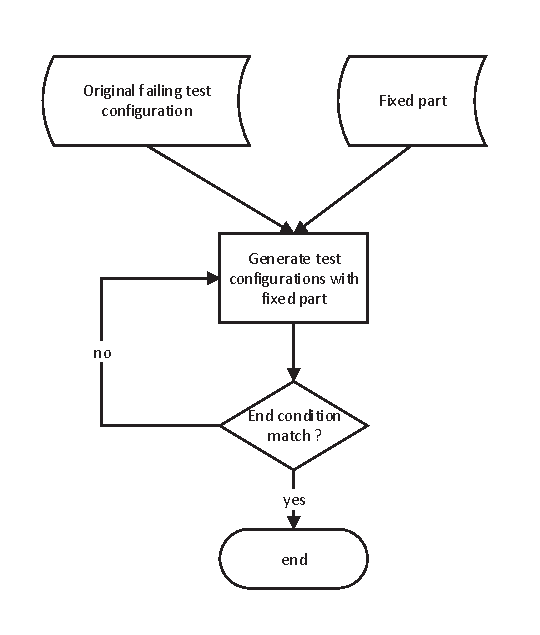
\epsfig{file=framework.eps, height=2.3in}
\caption{the overview of our approach.}
\end{figure}

This figure tell us when given a original failing test configuration and the fixed part, our approach will repeat generating test configurations which mutant the elements in the original test configuration except contain this fixed part until the end condition is matched.



1. Mutant other parts of the original test configurations

2. Execute the SUT under the test configuration make some  according to the result.

original failing test configuration.  and fixed part.

generate test configurations.

judge the based on reuslt

end. regenerate.

In a word, our approach takes a revalidation strategy when encouter different faults until we find a test case. Next we will discuss the two parts in detail.

\subsection{judge the result}
There are three condition we will end our algorithm:

1. If the generated test configuration passed during testing. This means that the fixed part we validated does not contain the failure-inducing elements, so we will send a message to tell the MFS identifying algorithm that this fixed part is a healthy part, and return this passing generated test configuration to these algorithms.

2.If the generated test configuration failed with the same faulty information as the original test configuration.


3.We cannot generate anymore test configurations contained this fixed part and diff from the original test configuration.

In this case, we didn't know which condition does this fixed part should be because we didn't find any test configuration that contain this part and either passed or failed with the same fault information. In this paper, we default set this fixed part as the failure-inducing . And return any test configuration generated.

In fact, to be efficiency, we set the repeat times as a fixed number, say 3 to be end as soon as possible.

Reversely, the only condition that we did not stop is that we encounter a different fault information as the original test configuration, for in that case we did not has enough information whether this fixed part is a failure-inducing part or not as the different fault information may be a masking effect.

\subsection{regenerate}
The regenerate step is to regenerate test configuration that contain the fixed part and does not contain any same elements in the remained part. The reason is that if so we can't not make sure the fixed part or the contained remained part is the failure-inducing part.

Further more, as we having set a fixed number, we can't running all the possible test configuration, so if we did not encounter the passed or the same fault, we will take some more test configuration instead all of them to test. As similar test configuration will trigger the same fault, so we vary them as different as possible to avoid the following condition:

all the regenerated test configuration trigger a fault that have a higher level that the original one.
The method we generate the test configuration it using random method. that is, using random number to take these unfixed part.

We generate as different as possible test cases for the tuple, to aviod some more MFSs that may mask this tuple. To do this we maintain a hash table to record the tuple and its corresponding test cases generated, each time we generate a random test case for this tuple, we will lookup this table to find if this test case is already generated, thus we will avoid generating redundancy test cases.

we will give simple example next to illustrate our approach. Take the fic as a example.

\subsection{simple example}


The approach, our approach is that,

if the algorithm want to get the result, we will put off the result, and generate another one.


generate test cases:


Five setup as follows:

Another note is that:

In detail, for FIC, TRT, OFOT, it can just use the original approach, that it each time test one tuple, and the we use our framework to assign this task.

For CTA, we can use our framework to choose a set of test cases for it to identify the MFS, like shykara do, but different from her work, we just not one test one time, we diff the test cases for different fault.


For SP, we can use our framework for him to generate test cases, it will test multiple tuples one time, and we just first for one fault, then another.

So  our comparison work is just compare the one fault, with a noise for the multiple faults.

\section{empirical studies}
To evaluate our approach, we take two open-source software as our subjects: HSQLDB and . HSQLDB is a pure-java data-base management software, and  is a . Both of them have a large support developers' forum. Further more as our approach is a framework that can bee seen as a for the MFS identifying algorithms, so that we afford them five algorithms: fic ofot trt cta sp.

There are three questions we want to figure our in this empirical studies:

Q1: does our framework reduce the number of MFSs and the degree of MFS?

Q2: does our framework can validate that MFSs exist masking effect.

Q3: does our framework the result is match the result in developer's forum.

\subsection{experiment set up}

\subsection{evaluation metrics}

\subsection{result and analysis}


\section{related works}
combinatorial testing has may factors, Nie give a survey, at some are focus,.

Identify MFS are

then consider the masking effect is , to my best knowledge, only one paper, unfortunately, it just consider the .

Ylimaz propose a work that is feedback driven combinatorial testing, different from our work, it first using CTA classify the possible MFS and then elimate them and generate new test cases to detect possible masked interaction in the next iteration. The difference is that the main focus of that work is to generate test cases that didn't omit some schemas that may be masked by other schemas. And our work is main focus on identifying the MFS and avoiding the masking effect.

\section{conclusion}

\section{The {\secit Body} of The Paper}
Typically, the body of a paper is organized
into a hierarchical structure, with numbered or unnumbered
headings for sections, subsections, sub-subsections, and even
smaller sections.  The command \texttt{{\char'134}section} that
precedes this paragraph is part of such a
hierarchy.\footnote{This is the second footnote.  It
starts a series of three footnotes that add nothing
informational, but just give an idea of how footnotes work
and look. It is a wordy one, just so you see
how a longish one plays out.} \LaTeX\ handles the numbering
and placement of these headings for you, when you use
the appropriate heading commands around the titles
of the headings.  If you want a sub-subsection or
smaller part to be unnumbered in your output, simply append an
asterisk to the command name.  Examples of both
numbered and unnumbered headings will appear throughout the
balance of this sample document.

Because the entire article is contained in
the \textbf{document} environment, you can indicate the
start of a new paragraph with a blank line in your
input file; that is why this sentence forms a separate paragraph.

\subsection{Type Changes and {\subsecit Special} Characters}
We have already seen several typeface changes in this sample.  You
can indicate italicized words or phrases in your text with
the command \texttt{{\char'134}textit}; emboldening with the
command \texttt{{\char'134}textbf}
and typewriter-style (for instance, for computer code) with
\texttt{{\char'134}texttt}.  But remember, you do not
have to indicate typestyle changes when such changes are
part of the \textit{structural} elements of your
article; for instance, the heading of this subsection will
be in a sans serif\footnote{A third footnote, here.
Let's make this a rather short one to
see how it looks.} typeface, but that is handled by the
document class file. Take care with the use
of\footnote{A fourth, and last, footnote.}
the curly braces in typeface changes; they mark
the beginning and end of
the text that is to be in the different typeface.

You can use whatever symbols, accented characters, or
non-English characters you need anywhere in your document;
you can find a complete list of what is
available in the \textit{\LaTeX\
User's Guide}\cite{Lamport:LaTeX}.

\subsection{Math Equations}
You may want to display math equations in three distinct styles:
inline, numbered or non-numbered display.  Each of
the three are discussed in the next sections.

\subsubsection{Inline (In-text) Equations}
A formula that appears in the running text is called an
inline or in-text formula.  It is produced by the
\textbf{math} environment, which can be
invoked with the usual \texttt{{\char'134}begin. . .{\char'134}end}
construction or with the short form \texttt{\$. . .\$}. You
can use any of the symbols and structures,
from $\alpha$ to $\omega$, available in
\LaTeX\cite{Lamport:LaTeX}; this section will simply show a
few examples of in-text equations in context. Notice how
this equation: \begin{math}\lim_{n\rightarrow \infty}x=0\end{math},
set here in in-line math style, looks slightly different when
set in display style.  (See next section).

\subsubsection{Display Equations}
A numbered display equation -- one set off by vertical space
from the text and centered horizontally -- is produced
by the \textbf{equation} environment. An unnumbered display
equation is produced by the \textbf{displaymath} environment.

Again, in either environment, you can use any of the symbols
and structures available in \LaTeX; this section will just
give a couple of examples of display equations in context.
First, consider the equation, shown as an inline equation above:
\begin{equation}\lim_{n\rightarrow \infty}x=0\end{equation}
Notice how it is formatted somewhat differently in
the \textbf{displaymath}
environment.  Now, we'll enter an unnumbered equation:
\begin{displaymath}\sum_{i=0}^{\infty} x + 1\end{displaymath}
and follow it with another numbered equation:
\begin{equation}\sum_{i=0}^{\infty}x_i=\int_{0}^{\pi+2} f\end{equation}
just to demonstrate \LaTeX's able handling of numbering.

\subsection{Citations}
Citations to articles \cite{bowman:reasoning,
clark:pct, braams:babel, herlihy:methodology},
conference proceedings \cite{clark:pct} or
books \cite{salas:calculus, Lamport:LaTeX} listed
in the Bibliography section of your
article will occur throughout the text of your article.
You should use BibTeX to automatically produce this bibliography;
you simply need to insert one of several citation commands with
a key of the item cited in the proper location in
the \texttt{.tex} file \cite{Lamport:LaTeX}.
The key is a short reference you invent to uniquely
identify each work; in this sample document, the key is
the first author's surname and a
word from the title.  This identifying key is included
with each item in the \texttt{.bib} file for your article.

The details of the construction of the \texttt{.bib} file
are beyond the scope of this sample document, but more
information can be found in the \textit{Author's Guide},
and exhaustive details in the \textit{\LaTeX\ User's
Guide}\cite{Lamport:LaTeX}.

This article shows only the plainest form
of the citation command, using \texttt{{\char'134}cite}.
This is what is stipulated in the SIGS style specifications.
No other citation format is endorsed or supported.

\subsection{Tables}
Because tables cannot be split across pages, the best
placement for them is typically the top of the page
nearest their initial cite.  To
ensure this proper ``floating'' placement of tables, use the
environment \textbf{table} to enclose the table's contents and
the table caption.  The contents of the table itself must go
in the \textbf{tabular} environment, to
be aligned properly in rows and columns, with the desired
horizontal and vertical rules.  Again, detailed instructions
on \textbf{tabular} material
is found in the \textit{\LaTeX\ User's Guide}.

Immediately following this sentence is the point at which
Table 1 is included in the input file; compare the
placement of the table here with the table in the printed
dvi output of this document.

\begin{table}
\centering
\caption{Frequency of Special Characters}
\begin{tabular}{|c|c|l|} \hline
Non-English or Math&Frequency&Comments\\ \hline
\O & 1 in 1,000& For Swedish names\\ \hline
$\pi$ & 1 in 5& Common in math\\ \hline
\$ & 4 in 5 & Used in business\\ \hline
$\Psi^2_1$ & 1 in 40,000& Unexplained usage\\
\hline\end{tabular}
\end{table}

To set a wider table, which takes up the whole width of
the page's live area, use the environment
\textbf{table*} to enclose the table's contents and
the table caption.  As with a single-column table, this wide
table will ``float" to a location deemed more desirable.
Immediately following this sentence is the point at which
Table 2 is included in the input file; again, it is
instructive to compare the placement of the
table here with the table in the printed dvi
output of this document.


\begin{table*}
\centering
\caption{Some Typical Commands}
\begin{tabular}{|c|c|l|} \hline
Command&A Number&Comments\\ \hline
\texttt{{\char'134}alignauthor} & 100& Author alignment\\ \hline
\texttt{{\char'134}numberofauthors}& 200& Author enumeration\\ \hline
\texttt{{\char'134}table}& 300 & For tables\\ \hline
\texttt{{\char'134}table*}& 400& For wider tables\\ \hline\end{tabular}
\end{table*}
% end the environment with {table*}, NOTE not {table}!

\subsection{Figures}
Like tables, figures cannot be split across pages; the
best placement for them
is typically the top or the bottom of the page nearest
their initial cite.  To ensure this proper ``floating'' placement
of figures, use the environment
\textbf{figure} to enclose the figure and its caption.

This sample document contains examples of \textbf{.eps}
and \textbf{.ps} files to be displayable with \LaTeX.  More
details on each of these is found in the \textit{Author's Guide}.

\begin{figure}
\centering
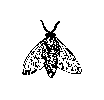
\epsfig{file=fly.eps}
\caption{A sample black and white graphic (.eps format).}
\end{figure}

\begin{figure}
\centering
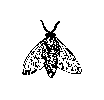
\epsfig{file=fly.eps, height=1in, width=1in}
\caption{A sample black and white graphic (.eps format)
that has been resized with the \texttt{epsfig} command.}
\end{figure}


As was the case with tables, you may want a figure
that spans two columns.  To do this, and still to
ensure proper ``floating'' placement of tables, use the environment
\textbf{figure*} to enclose the figure and its caption.
and don't forget to end the environment with
{figure*}, not {figure}!

\begin{figure*}
\centering
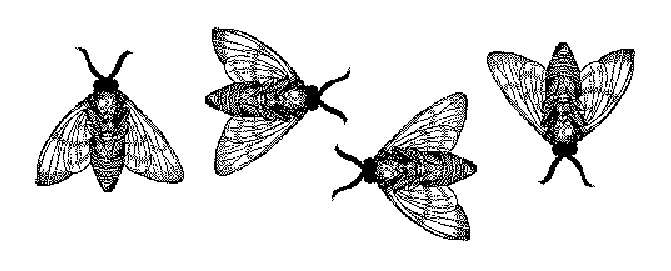
\epsfig{file=flies.eps}
\caption{A sample black and white graphic (.eps format)
that needs to span two columns of text.}
\end{figure*}

Note that either {\textbf{.ps}} or {\textbf{.eps}} formats are
used; use
the \texttt{{\char'134}epsfig} or \texttt{{\char'134}psfig}
commands as appropriate for the different file types.

\begin{figure}
\centering
\psfig{file=rosette.ps, height=1in, width=1in,}
\caption{A sample black and white graphic (.ps format) that has
been resized with the \texttt{psfig} command.}
\vskip -6pt
\end{figure}

\subsection{Theorem-like Constructs}
Other common constructs that may occur in your article are
the forms for logical constructs like theorems, axioms,
corollaries and proofs.  There are
two forms, one produced by the
command \texttt{{\char'134}newtheorem} and the
other by the command \texttt{{\char'134}newdef}; perhaps
the clearest and easiest way to distinguish them is
to compare the two in the output of this sample document:

This uses the \textbf{theorem} environment, created by
the\linebreak\texttt{{\char'134}newtheorem} command:
\newtheorem{theorem}{Theorem}
\begin{theorem}
Let $f$ be continuous on $[a,b]$.  If $G$ is
an antiderivative for $f$ on $[a,b]$, then
\begin{displaymath}\int^b_af(t)dt = G(b) - G(a).\end{displaymath}
\end{theorem}

The other uses the \textbf{definition} environment, created
by the \texttt{{\char'134}newdef} command:
\begin{definition}
If $z$ is irrational, then by $e^z$ we mean the
unique number which has
logarithm $z$: \begin{displaymath}{\log e^z = z}\end{displaymath}
\end{definition}

Two lists of constructs that use one of these
forms is given in the
\textit{Author's  Guidelines}.

There is one other similar construct environment, which is
already set up
for you; i.e. you must \textit{not} use
a \texttt{{\char'134}newdef} command to
create it: the \textbf{proof} environment.  Here
is a example of its use:
\begin{proof}
Suppose on the contrary there exists a real number $L$ such that
\begin{displaymath}
\lim_{x\rightarrow\infty} \frac{f(x)}{g(x)} = L.
\end{displaymath}
Then
\begin{displaymath}
l=\lim_{x\rightarrow c} f(x)
= \lim_{x\rightarrow c}
\left[ g{x} \cdot \frac{f(x)}{g(x)} \right ]
= \lim_{x\rightarrow c} g(x) \cdot \lim_{x\rightarrow c}
\frac{f(x)}{g(x)} = 0\cdot L = 0,
\end{displaymath}
which contradicts our assumption that $l\neq 0$.
\end{proof}

Complete rules about using these environments and using the
two different creation commands are in the
\textit{Author's Guide}; please consult it for more
detailed instructions.  If you need to use another construct,
not listed therein, which you want to have the same
formatting as the Theorem
or the Definition\cite{salas:calculus} shown above,
use the \texttt{{\char'134}newtheorem} or the
\texttt{{\char'134}newdef} command,
respectively, to create it.

\subsection*{A {\secit Caveat} for the \TeX\ Expert}
Because you have just been given permission to
use the \texttt{{\char'134}newdef} command to create a
new form, you might think you can
use \TeX's \texttt{{\char'134}def} to create a
new command: \textit{Please refrain from doing this!}
Remember that your \LaTeX\ source code is primarily intended
to create camera-ready copy, but may be converted
to other forms -- e.g. HTML. If you inadvertently omit
some or all of the \texttt{{\char'134}def}s recompilation will
be, to say the least, problematic.

\section{Conclusions}
This paragraph will end the body of this sample document.
Remember that you might still have Acknowledgments or
Appendices; brief samples of these
follow.  There is still the Bibliography to deal with; and
we will make a disclaimer about that here: with the exception
of the reference to the \LaTeX\ book, the citations in
this paper are to articles which have nothing to
do with the present subject and are used as
examples only.
%\end{document}  % This is where a 'short' article might terminate

%ACKNOWLEDGMENTS are optional
\section{Acknowledgments}
This section is optional; it is a location for you
to acknowledge grants, funding, editing assistance and
what have you.  In the present case, for example, the
authors would like to thank Gerald Murray of ACM for
his help in codifying this \textit{Author's Guide}
and the \textbf{.cls} and \textbf{.tex} files that it describes.

%
% The following two commands are all you need in the
% initial runs of your .tex file to
% produce the bibliography for the citations in your paper.
\bibliographystyle{abbrv}
\bibliography{sigproc}  % sigproc.bib is the name of the Bibliography in this case
% You must have a proper ".bib" file
%  and remember to run:
% latex bibtex latex latex
% to resolve all references
%
% ACM needs 'a single self-contained file'!
%
%APPENDICES are optional
%\balancecolumns
\appendix
%Appendix A
\section{Headings in Appendices}
The rules about hierarchical headings discussed above for
the body of the article are different in the appendices.
In the \textbf{appendix} environment, the command
\textbf{section} is used to
indicate the start of each Appendix, with alphabetic order
designation (i.e. the first is A, the second B, etc.) and
a title (if you include one).  So, if you need
hierarchical structure
\textit{within} an Appendix, start with \textbf{subsection} as the
highest level. Here is an outline of the body of this
document in Appendix-appropriate form:
\subsection{Introduction}
\subsection{The Body of the Paper}
\subsubsection{Type Changes and  Special Characters}
\subsubsection{Math Equations}
\paragraph{Inline (In-text) Equations}
\paragraph{Display Equations}
\subsubsection{Citations}
\subsubsection{Tables}
\subsubsection{Figures}
\subsubsection{Theorem-like Constructs}
\subsubsection*{A Caveat for the \TeX\ Expert}
\subsection{Conclusions}
\subsection{Acknowledgments}
\subsection{Additional Authors}
This section is inserted by \LaTeX; you do not insert it.
You just add the names and information in the
\texttt{{\char'134}additionalauthors} command at the start
of the document.
\subsection{References}
Generated by bibtex from your ~.bib file.  Run latex,
then bibtex, then latex twice (to resolve references)
to create the ~.bbl file.  Insert that ~.bbl file into
the .tex source file and comment out
the command \texttt{{\char'134}thebibliography}.
% This next section command marks the start of
% Appendix B, and does not continue the present hierarchy
\section{More Help for the Hardy}
The sig-alternate.cls file itself is chock-full of succinct
and helpful comments.  If you consider yourself a moderately
experienced to expert user of \LaTeX, you may find reading
it useful but please remember not to change it.
%\balancecolumns % GM June 2007
% That's all folks!
\end{document}
